\documentclass[11pt,a4paper]{report}

% packages
\usepackage[left=20mm, right=15mm, top=10mm, bottom=15mm]{geometry}
\usepackage{tocloft}
\usepackage{graphicx}
\usepackage{subcaption}
\usepackage{amsmath}
\usepackage{setspace}
\usepackage{makecell}
\usepackage[utf8]{inputenc}
\usepackage[english]{babel}
\usepackage{amsthm}
\usepackage{arevmath}
\usepackage[noend]{algpseudocode}
\usepackage{amssymb}
\usepackage{algorithm2e}
\usepackage{hyperref}

% configuration
\theoremstyle{definition}
\newtheorem{definition}{Definition}[section]
\theoremstyle{remark}
\newtheorem*{remark}{Remark}
\hypersetup{
    colorlinks=true,
    linkcolor=blue,
    filecolor=magenta,      
    urlcolor=cyan
}


\begin{document}

    %set up the titles page
   \begin{titlepage}
        \begin{center}
        \vspace*{1cm}
            
        \Huge
        \textbf{SOEN-6011 PROJECT}
            
        \vspace{0.5cm}
        \LARGE
        Eternity
            
        \vspace{1.5cm}
            
        \textbf{Akhil Sharma}
            
        \vfill
            
        Implementation of the Power Function.
            
        \vspace{15cm}
        \end{center}
    \end{titlepage}
    \tableofcontents
    \clearpage
    
    \section{Introduction}
    The objective of this medium-sized scientific software engineering project is to implement the power function while approaching the problem from first principles. Tasks like \textbf{documenting}, \textbf{versioning}, and \textbf{testing} are considered first class citizens.
    
    \vspace{0.75cm}
    
    This report will first discuss about the power function. This is followed by defining the requirements for the system. Defining the requirements will also impose a restriction on the scope of the project. This is followed by comparing different algorithms for calculating the power function and selecting the most efficient based on the time complexity. Next, the method is implemented from scratch in java along with a simple textual user interface. The report also discusses the use of various tools like the debugger and the type check. Finally, the report will discuss the process of testing the system.
    
    \vspace{0.75cm}
    
    As required by the project description, this report was typeset using \LaTeX . The \LaTeX source was tested online at \href{https://overleaf.com}{Overleaf} and offline on MikTex for windows.
    
    \vspace{0.75cm}
    
    The source code for the project is hosted on \href{https://github.com/akhil-sharma/soen6011-eternity.git}{GitHub} 
    
    \vspace{0.75cm}
    
    The terms Project, System, Software system, Eternity all refer to the same thing.
    
    \chapter{Power Function}
    
        \begin{definition}
            The \textbf{power function} is defined as the function that takes any numbers $x$ and $y$ as input, raises $x$ to $y$, and returns $x^y$ as output.
        \end{definition}
    
        The power function is a transcendental function and cannot be expressed in terms of a finite sequence of the algebraic operations of raising to a power, division, multiplication, addition, subtraction, and root extraction \href{https://en.wikipedia.org/wiki/Transcendental_function}{wikipedia}.
        
        All the exponentiation rules are applicable here.
        
        \section{Domain and Co-domain}
        The domains and co-domains of $x$ and $y$ vary as follows \cite{algorithms}:
        
        \begin{itemize}
            \item If \textbf{base $x$ is a positive real number}, then $y$ belongs to the set of all reals numbers.
            
            The corresponding range is the set of all positive real numbers.
            
            \item If \textbf{base $x$ is zero}, then $y$ belongs to the set of non-negative real numbers.
            
            This is because a negative $y$ would lead to division by zero.
            
            \item If \textbf{base $x$ is negative}, then $y$ may only have to certain values:

                    \begin{itemize}
                        \item $y$ \textbf{may be} any integer.
                        
                        \item $y$ \textbf{may be} a fraction of the form $a/b$ where \emph{b} is odd.
                        
                        \item $y$ \textbf{may not be} a fraction of the form $a/b$ where \emph{b} is even.
                        
                        \item $y$ \textbf{may not be} an irrational number. 
                        
                    \end{itemize}
            
        \end{itemize}
        
        \section{Examples}
        Let's look a few examples:
        
        Any number raised to the power one results in the same number, $2^1 \, = \, 2 \,$ .
        
        Two to the power three means two times two times two or $2^3 \, = \, 8 \,$ .
        
        Zero raised to any positive power is 0.
        
        Zero raised to power zero is 1.
        
        For negative powers, $x ^ {-y} = 1 / x^y$. So, $2 ^ {-1} = 1 / 2^1 = 0.5$
        
        
        
        \section{Context of use Model}
            The context of use is a description of the conditions under which the software system will be used under the normal working circumstances. 
            A context of use model is a useful tool to explore and understand the details and boundaries of a project. \cite{context diagrams}
            
            There is currently no standard for representing the context of use. A context diagram is however a suitable candidate for mind mapping. 
            
            Fig 1. is a context diagram for this project built using the \href{https://gitmind.com/}{GitMind tool}. It focuses on the users of the systems and the environments where this system will be operated. The users block is subdivided into blocks representing the potential users of the system and their requirements for effective and efficient completion of their responsibilities.
            
            The environment block explores the different system environments needed to perform different tasks. In particular, the developers, testers and, maintainer require a Technical environment. The end-user however doesn't require anything more than the general environment.
        
            \begin{figure}[htbp]
                \centering
                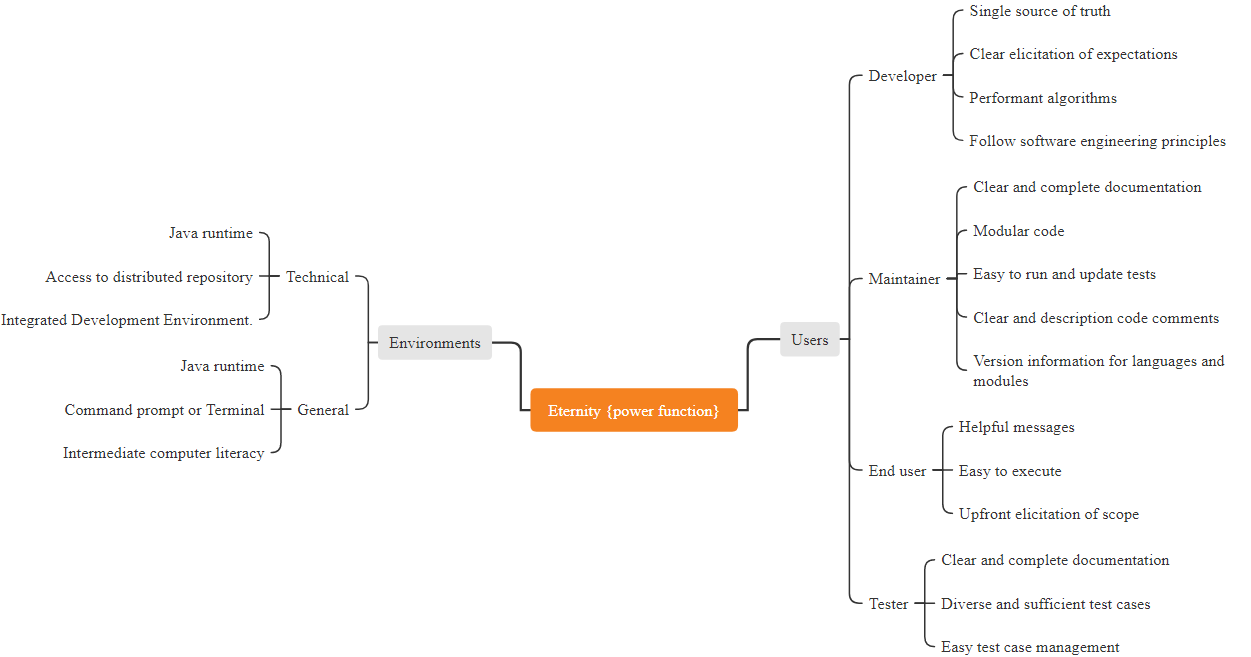
\includegraphics[width=\linewidth]{Context_of_use.PNG}
                \caption{Context of use for Eternity.}
                \label{fig:context_of_use}
            \end{figure}
        
    \chapter{Requirements}
        This chapter lists the software requirements using the format outlined in the ISO/IEC/IEEE 29148 sections 5.2.4 to 5.2.7 (“ISO/IEC/IEEE International Standard - Systems and Software Engineering -- Life Cycle Processes -- Requirements Engineering,” 2018). 
        The following meta data is associated with each requirement:
    
        \begin{description}
            \item[ID] This string uniquely identifies the requirement.
            \item[VERSION] This indicates the number of times a requirement has been updated.
            \item[PRIORITY] This string indicates the importance of implementing this requirement for the minimum viable product. Priority may be one of HIGH, AVERAGE, or LOW.
            \item[TYPE] This string indicates whether the requirement is functional or non-functional in nature.        
        \end{description}
        
        The requirements were managed using the Jira dashboard. See figure \ref{fig:jira_requirement_management}.
        
        \vspace{3em}
    
        % Tables for requirements.
        % Requirement 1
        \begin{table}[ht]
        \centering
            \begin{tabular}{cccc} % ll can be replace with c. | is a table line
                \textbf{ID} & \textbf{VERSION} & \textbf{PRIORITY} & \textbf{TYPE}\\
                        R1  &           1      &           HIGH    &      NON-FUNCTIONAL\\
                \hline
                \multicolumn{4}{l}{Eternity shall execute on any device with JVM.}
            \end{tabular}
            \caption{Requirement 1}
            \label{tab:table-requirements-1}
        \end{table}
        \vspace{3em}
        
        % Requirement 2
        \begin{table}[ht]
        \centering
            \begin{tabular}{cccc} % ll can be replace with c. | is a table line
                \textbf{ID} & \textbf{VERSION} & \textbf{PRIORITY} & \textbf{TYPE}\\
                        R2  &           1      &           HIGH    &      FUNCTIONAL\\
                \hline
                \multicolumn{4}{l}{Eternity shall allow multiple calculations per session}
            \end{tabular}
            \caption{Requirement 2}
            \label{tab:table-requirements-2}
        \end{table}
        \vspace{3em}
        
        % Requirement 3
        \begin{table}[ht]
        \centering
            \begin{tabular}{cccc} % ll can be replace with c. | is a table line
                \textbf{ID} & \textbf{VERSION} & \textbf{PRIORITY} & \textbf{TYPE}\\
                        R3  &           1      &           HIGH    &      NON-FUNCTIONAL\\
                \hline
                \multicolumn{4}{l}{Eternity shall be developed with maintainability in mind.}
            \end{tabular}
            \caption{Requirement 3}
            \label{tab:table-requirements-3}
        \end{table}
        \vspace{3em}

        % Requirement 4
        \begin{table}[ht]
        \centering
            \begin{tabular}{cccc} % ll can be replace with c. | is a table line
                \textbf{ID} & \textbf{VERSION} & \textbf{PRIORITY} & \textbf{TYPE}\\
                        R4  &           1      &           HIGH    &      NON-FUNCTIONAL\\
                \hline
                \multicolumn{4}{l}{Eternity shall be modular and testable.}
            \end{tabular}
            \caption{Requirement 4}
            \label{tab:table-requirements-4}
        \end{table}
        \vspace{3em}
        
        % Requirement 5
        \begin{table}[ht]
        \centering
            \begin{tabular}{cccc} % ll can be replace with c. | is a table line
                \textbf{ID} & \textbf{VERSION} & \textbf{PRIORITY} & \textbf{TYPE}\\
                        R5  &           1      &           HIGH    &      NON-FUNCTIONAL\\
                \hline
                \multicolumn{4}{l}{Eternity shall have a simple user interface to increase usability.}
            \end{tabular}
            \caption{Requirement 5}
            \label{tab:table-requirements-5}
        \end{table}
        \vspace{3em}
        
        % Requirement 6
        \begin{table}[ht]
        \centering
            \begin{tabular}{cccc} % ll can be replace with c. | is a table line
                \textbf{ID} & \textbf{VERSION} & \textbf{PRIORITY} & \textbf{TYPE}\\
                        R6  &           1      &           HIGH    &      FUNCTIONAL\\
                \hline
                \multicolumn{4}{l}{Eternity shall allow only integer values of $y$ when calculating $x^y$.}
            \end{tabular}
            \caption{Requirement 6}
            \label{tab:table-requirements-6}
        \end{table}
        \vspace{3em}
        
        % Requirement 7
        \begin{table}[ht]
        \centering
            \begin{tabular}{cccc} % ll can be replace with c. | is a table line
                \textbf{ID} & \textbf{VERSION} & \textbf{PRIORITY} & \textbf{TYPE}\\
                        R7  &           1      &           HIGH    &      FUNCTIONAL\\
                \hline
                \multicolumn{4}{l}{Eternity shall allow all real values for $x$ when calculating $x^y$.}
            \end{tabular}
            \caption{Requirement 7}
            \label{tab:table-requirements-7}
        \end{table}
        \vspace{3em}
        
        % Requirement 8
        \begin{table}[ht]
        \centering
            \begin{tabular}{cccc} % ll can be replace with c. | is a table line
                \textbf{ID} & \textbf{VERSION} & \textbf{PRIORITY} & \textbf{TYPE}\\
                        R8  &           1      &           HIGH    &      NON-FUNCTIONAL\\
                \hline
                \multicolumn{4}{l}{Eternity shall provide a help menu for users.}
            \end{tabular}
            \caption{Requirement 8}
            \label{tab:table-requirements-8}
        \end{table}
        \vspace{3em}
        
        % Requirement 9
        \begin{table}[ht]
        \centering
            \begin{tabular}{cccc} % ll can be replace with c. | is a table line
                \textbf{ID} & \textbf{VERSION} & \textbf{PRIORITY} & \textbf{TYPE}\\
                        R9  &           1      &           HIGH    &      NON-FUNCTIONAL\\
                \hline
                \multicolumn{4}{l}{Eternity shall provide Javadoc documentation.}
            \end{tabular}
            \caption{Requirement 9}
            \label{tab:table-requirements-9}
        \end{table}
        \vspace{3em}
        
        % Requirement 10
        \begin{table}[ht]
        \centering
            \begin{tabular}{cccc} % ll can be replace with c. | is a table line
                \textbf{ID} & \textbf{VERSION} & \textbf{PRIORITY} & \textbf{TYPE}\\
                        R10  &           1      &           HIGH    &      FUNCTIONAL\\
                \hline
                \multicolumn{4}{l}{Eternity shall use optimal algorithms.}
            \end{tabular}
            \caption{Requirement 10}
            \label{tab:table-requirements-10}
        \end{table}
        \vspace{3em}
        
        % Requirement 11
        \begin{table}[ht]
        \centering
            \begin{tabular}{cccc} % ll can be replace with c. | is a table line
                \textbf{ID} & \textbf{VERSION} & \textbf{PRIORITY} & \textbf{TYPE}\\
                        R11  &           1      &           HIGH    &      FUNCTIONAL\\
                \hline
                \multicolumn{4}{l}{Eternity shall not allow $x$ to be 0 when $y$ is negative.}
            \end{tabular}
            \caption{Requirement 11}
            \label{tab:table-requirements-11}
        \end{table}
        \vspace{3em}
        
        % Requirement 12
        \begin{table}[ht]
        \centering
            \begin{tabular}{cccc} % ll can be replace with c. | is a table line
                \textbf{ID} & \textbf{VERSION} & \textbf{PRIORITY} & \textbf{TYPE}\\
                        R12  &           1      &           HIGH    &      FUNCTIONAL\\
                \hline
                \multicolumn{4}{l}{Eternity shall return 1 when the power is 0.}
            \end{tabular}
            \caption{Requirement 12}
            \label{tab:table-requirements-12}
        \end{table}
        \vspace{3em}
        
        % Requirement 13
        \begin{table}[ht]
        \centering
            \begin{tabular}{cccc} % ll can be replace with c. | is a table line
                \textbf{ID} & \textbf{VERSION} & \textbf{PRIORITY} & \textbf{TYPE}\\
                        R13  &           1      &           HIGH    &      FUNCTIONAL\\
                \hline
                \multicolumn{4}{l}{Eternity shall return $x$ when $y$ = 1 in $x^y$.}
            \end{tabular}
            \caption{Requirement 13}
            \label{tab:table-requirements-13}
        \end{table}
        \vspace{3em}
        
        % Requirement 14
        \begin{table}[t]
        \centering
            \begin{tabular}{cccc} % ll can be replace with c. | is a table line
                \textbf{ID} & \textbf{VERSION} & \textbf{PRIORITY} & \textbf{TYPE}\\
                        R14  &           1      &           LOW    &      FUNCTIONAL\\
                \hline
                \multicolumn{4}{l}{Eternity will maintain a history of previous operations.}
            \end{tabular}
            \caption{Requirement 14}
            \label{tab:table-requirements-14}
        \end{table}
        
    \chapter{Algorithm}
        There exist a few algorithms for calculating the power function. However, requirements \ref{tab:table-requirements-6} and \ref{tab:table-requirements-7} significantly reduce the scope this project.
        We will consider two algorithms for Eternity, the repeated multiplication or iterative solution and, the divide and conquer solution.
        When discussing these algorithms we will assume that the power $y$ is positive since the solution for negative $y$ can be derived trivially from this value.
         
        \section{Iterative Solution (Naive approach)} % algorithm level
        	The iterative solution is the simplest way solve this problem. The calculation of $x^y$ involves multiplying \emph{X} with itself exactly $y$ times.
        	For example, $2^3 \, = \, 2 \, * \, 2 \, * \, 2 \, = \, 8$.
        	
        	\subsection{Pseudocode}
            	\begin{description}
                	\item [Input]: Numbers $x$ and $y$ where $x$ is a real number and $y$ is a positive integer.
                	\item [Output]: Return the value power function $x^y$.
            	\end{description}
            	
            	\begin{algorithm}
                	\SetKwInput{function}{Function}
                	\function{$power\_incremental$($x, y$)}
                	    $power \gets 1$\;
                	    \While{$y > 0$}{
                	        $power \gets power * x$\;
                	        $y = y - 1$\;
                	    }
                	    \Return {$power$}\;
                \caption{Power function using repeated multiplication (Naive).}
                \label{alg:power-incremental}
            	\end{algorithm}
            	
            \subsection{Complexity}
            This is a relatively straightforward algorithm and runs in linear time. This results to a time complexity of $O(n)$ where $n$ is the magnitude of power $y$.
        
        \clearpage
        \section{Divide and Conquer}
            In the \textbf{Divide and Conquer} approach the problem is defined recursively as follows:
            $$power(x, \, y) = power(x, \, y \, / \, 2) \, * \, power(x, \, y \, / \, 2), \, if \, y \, is \, even$$
            $$power(x, \, y) = x \, * \, power(x, \, y \, / \, 2) \, * \, power(x, \, y \, / \, 2), \, if \, y \, is \, odd$$
        
            Here, the problem is being divided into a sub-problem which is half the size of the original problem until the base case is reached where $y \, = \, 1.$
        
            \subsection{Pseudocode}
            	\begin{description}
                	\item [Input]: Numbers $x$ and $y$ where $x$ is a real number and $y$ is a positive integer.
                	\item [Output]: Return the value power function $x^y$.
            	\end{description}
            	
            	\begin{algorithm}
                	\SetKwInput{function}{Function}
                	\function{$power\_divide\_and\_conquer$($x, y$)}
                        \If{$y = 0$}{
                            \Return {1}\;
                        }
                        
                        $pow \gets power\_divide\_and\_conquer(x, y / 2)$\;
                        
                        \If{$y$ is odd}{
                            \Return {$x\,*\, pow \,*\, pow$}\;
                        }{
                            \Return {$pow\,*\,pow$}\;
                        }
                \caption{Power function using divide and conquer.}
                \label{alg:power-divide-and-conquer}
            	\end{algorithm}
            
            \subsection{Complexity}
                Since this algorithm continuously divides the problem in half we get the time complexity of $\mathcal{O}(\log n)$ where $n$ is the magnitude of $y$.
            
        
        \section{Final Selection}
            By comparing the above algorithms, it is clear that the algorithm \ref{alg:power-divide-and-conquer} \textbf{divide and conquer} performs better than algorithm \ref{alg:power-incremental} \textbf{direct approach}. As a result, Eternity will implement the second algorithm or algorithm \ref{alg:power-divide-and-conquer}.
        
        \clearpage
        
        \section{Pseudocode Style Selection}
            There exist a number of styles for writing pseudocodes. Mind mapping was used to determine the style that suits our purpose. See figure \ref{fig:pseudocode_mindmap}.
            
            The pseudocode style provided by the algorithm2e \LaTeX package was determined to be best suited since it provides a format which is very similar to the c-style or java-style and capable of representing much detail.
            
            This style was preferred over the python style since it is \textbf{closer in distance} to the java code in the repository.
            
            \begin{figure}[htbp]
                \centering
                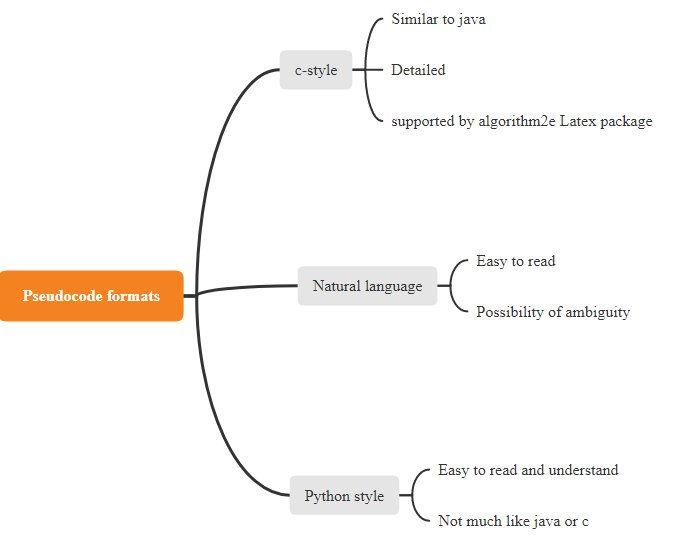
\includegraphics[width=0.75\linewidth]{pseudocode_mindmap.PNG}
                \caption{Mind Mapping to determine the pseudocode style.}
                \label{fig:pseudocode_mindmap}
            \end{figure}
        
    
    \chapter{Problem}
        The project is implemented from scratch in Java. The term “scratch” means that, apart from the functions related to input, output, arithmetic, and user interface design, your implementation does not use any built-in or library functions provided by Java.
        
        The project uses \href{https://google.github.io/styleguide/javaguide.html}{Google's java style guide} since most of the popular style guides are derived from it.
        
        Eternity uses a textual interface since seemed appropriate for a project of this scope. The developer's inexperience in building graphical user interface also contributed to this decision.
        
        \section{Requirements Management}
        During the development of Eternity the requirements were managed using Jira. Figure \ref{fig:jira_requirement_management} the Jira dashboard for requirements.
        
            \begin{figure}[htbp]
                \centering
                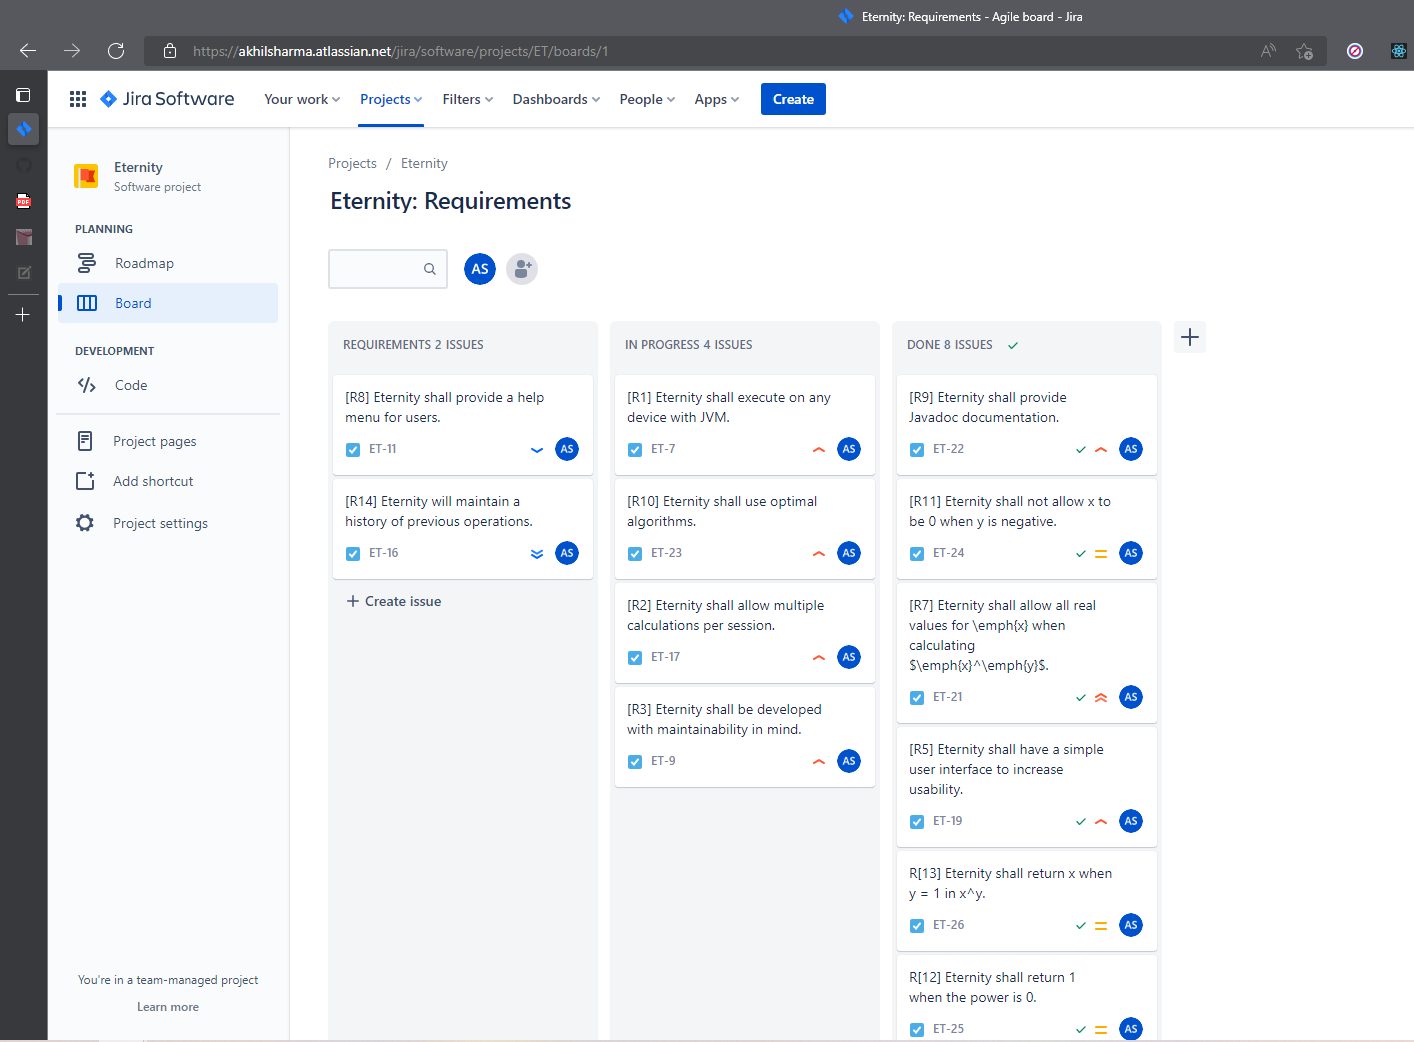
\includegraphics[width=\linewidth]{requirements_management.PNG}
                \caption{Requirements management in jira.}
                \label{fig:jira_requirement_management}
            \end{figure}
        
        \section{Debugger}
        Eternity uses the open-source Debugger for Java [] built into visual studio code.
        It is a lightweight java debugger based on Java Debug Server which extends the Language Support for Java by Red Hat. It allows users to debug Java code using Visual Studio Code (VS Code). It has a number of features like:
            \begin{itemize}
                \item Launch/Attach
                \item Breakpoints/Conditional Breakpoints/Logpoints
                \item Exceptions
                \item Pause and Continue
                \item Step In/Out/Over
                \item Variables
                \item Callstacks
                \item Threads
                \item Debug console
                \item Evaluation
                \item Hot Code Replace
            \end{itemize}
        
        Figure \ref{fig:vs_code_debugger} shows the debugger in action. It is an open-source project backed by tech giants like Microsoft. It offer a very granular control over the process and can be configured as needed. It comes pre-installed with VS Code and needs little knowledge to get started with. All these factors made it the debugger of choice for me.
    
            \begin{figure}[htbp]
                \centering
                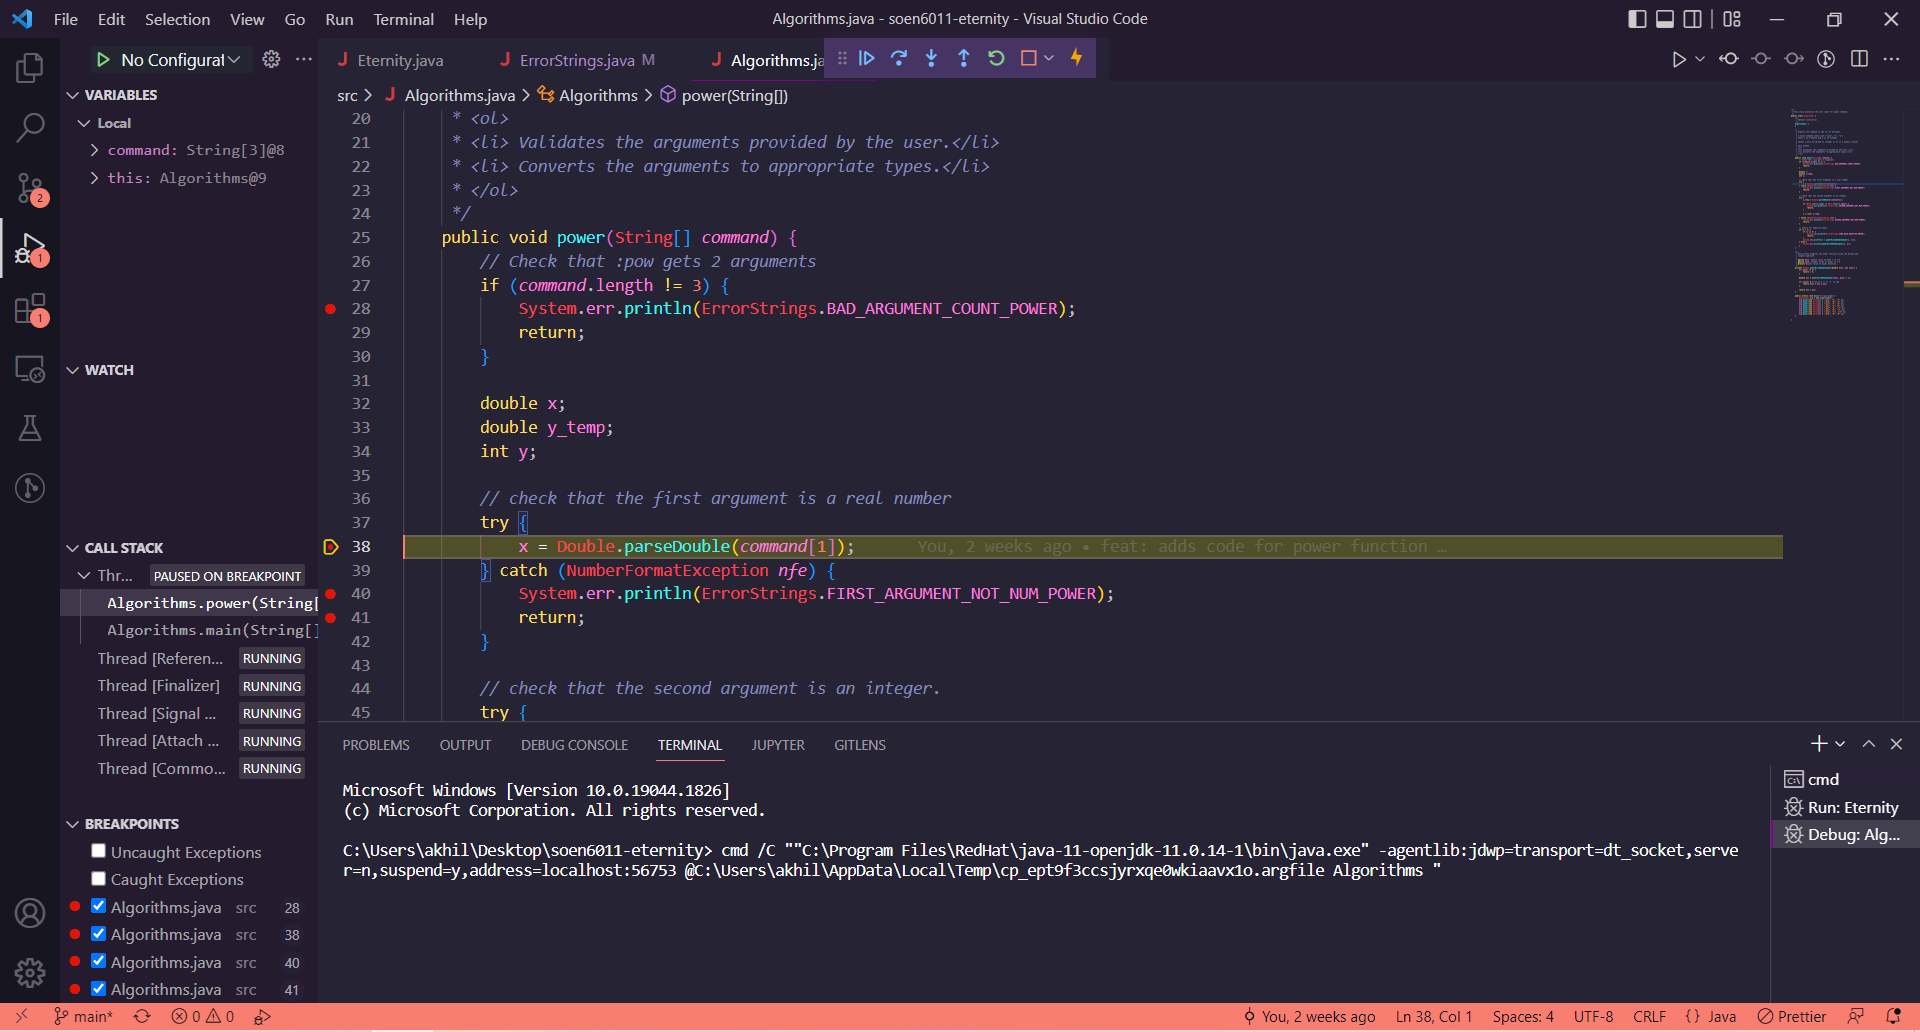
\includegraphics[width=\linewidth]{debugger.PNG}
                \caption{VS Code debugger in action.}
                \label{fig:vs_code_debugger}
            \end{figure}
            
        \section{Checkstyle}
        \textbf{Checkstyle} is a convenient tool to apply Checkstyle rules to your Java source code so you can see the style issues and fix them on the fly. It automates the process of checking your Java code so the developer is freed while keeping your format correct. The checkstyle plugin for vs code also includes the Google style guide built-in to it make the whole process very smooth. Figure \ref{fig:vs_code_checkstyle} show the checkstyle tool in action.
        
            \begin{figure}[htbp]
                \centering
                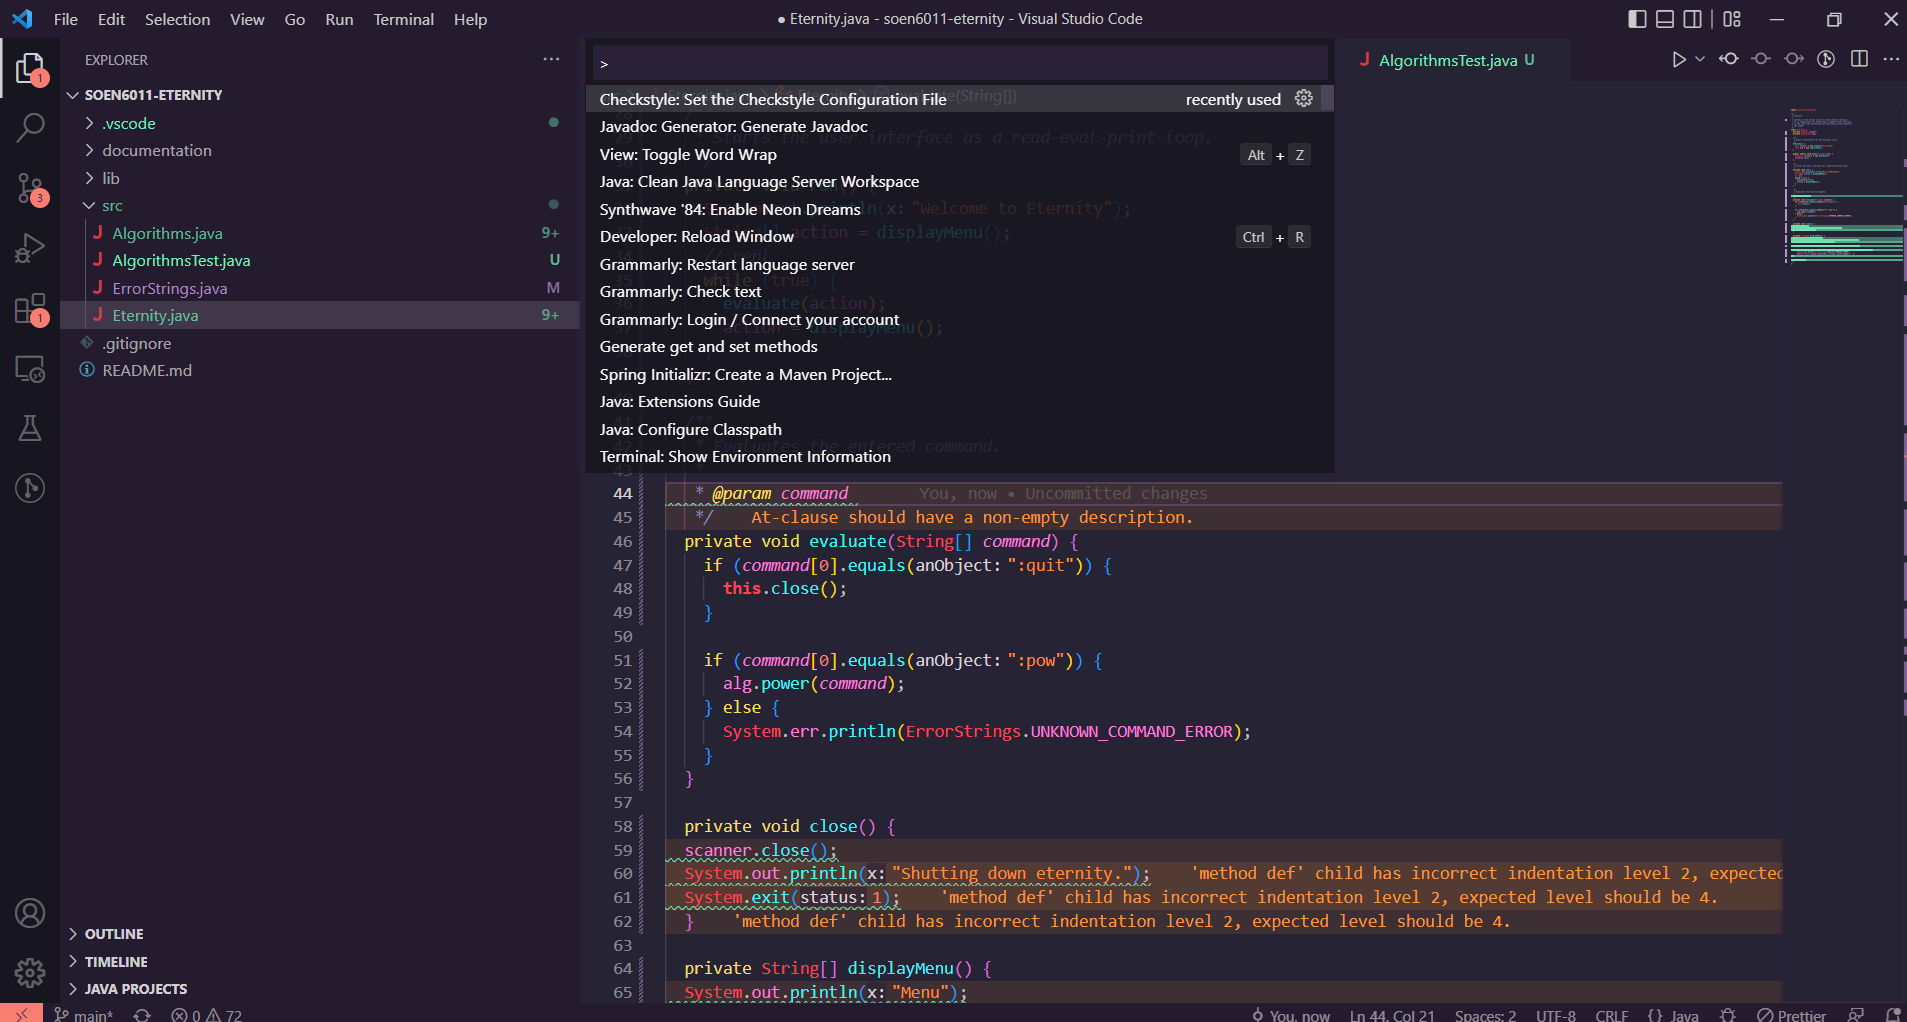
\includegraphics[width=\linewidth]{checkstyle.PNG}
                \caption{Running checkstyle on code using the built-in Google style guide.}
                \label{fig:vs_code_checkstyle}
            \end{figure}
        
        \section{Quality Attributes Management}
        A significant consideration went into managing the quality attributes of Eternity. Some of these attributes and associated actions mentioned below.
            \begin{itemize}
                \item \textbf{Space efficiency}: Eternity evaluates all commands on the fly without saving artifact from the previous executions. Variable creation minimized when possible. Efforts have been made to ensure graceful exiting by closing streams before quitting.
                
                \item \textbf{Portability}: Eternity uses an unmanaged directory structure with out any build tool written in java from scratch. This results in high portability as the code will compile and execute on any device which which has JVM installed. Special care has been taken to prevent dependence on any IDE or operating system as well.
                
                \item \textbf{Maintainability}: Many actions have been taken to make the project maintainable. Extensive use of javadoc comments, breaking down functionality into separate files, maintaining a commit history using distributed version management are some of these actions. In addition, each command is validated and handled by a separate file making it trivial to add new commands.
                
                \item \textbf{Correctness}: The correctness has be ensured by adding a sufficient number of test cases for unit testing the commands (here, power). 
                
                \item \textbf{Time efficiency}: The algorithm used by Eternity is based on the `divide and conquer approach` and was selected due to its superior time complexity compare to the naive algorithms. This contributes to improving the time efficiency of the project.
                
                \item \textbf{Robustness}: Extensive unit testing, \textbf{exception handling} help make eternity robust.
                
                \item \textbf{Usability}: Eternity offers a very simple textual interface which display the available commands to the user. In addition it also displays \textbf{helpful messages (errors or otherwise)} to make sure that the user is never in the dark. User is also greeted with a welcome and an exit message to provide the boundary to the user experience. All these efforts contribute to the usability of the product.

            \end{itemize}
    
    \chapter {Testing}
    Testing is necessary to ensure the correctness and robustness of the software system. Unit testing for Eternity was done using the JUnit 4 library. Expiration of Jira trial period motivated the use of Microsoft Excel for the purpose of Test case management. Figure \ref{fig:test_case_management} shows a snapshot of the test case management workbook.
    
    The association between Test cases and the requirements were also recorded.
    
        \begin{figure}[htbp]
            \centering
            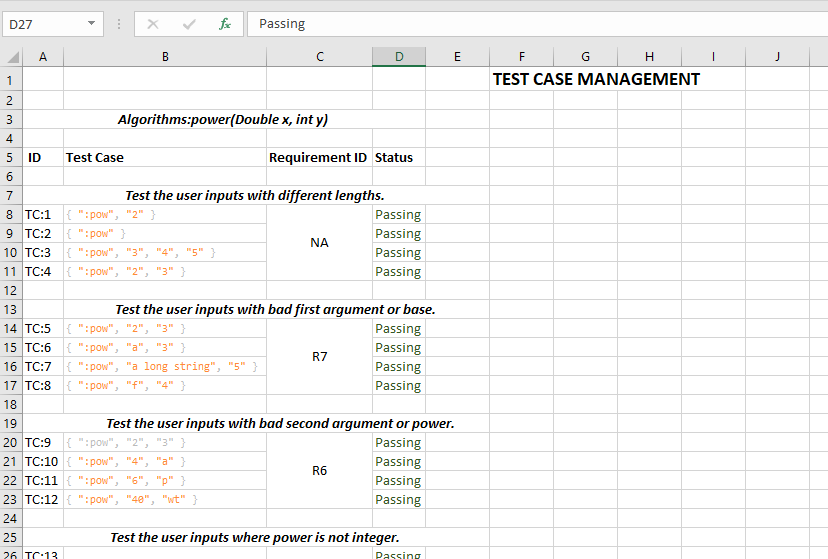
\includegraphics[width=\linewidth]{test_case_management.PNG}
            \caption{Test case management using excel.}
            \label{fig:test_case_management}
        \end{figure}
        
    Figure \ref{fig:passed_test_cases} demonstrates the execution of the JUnit-4 test cases in VS Code.
        
        \begin{figure}[htbp]
            \centering
            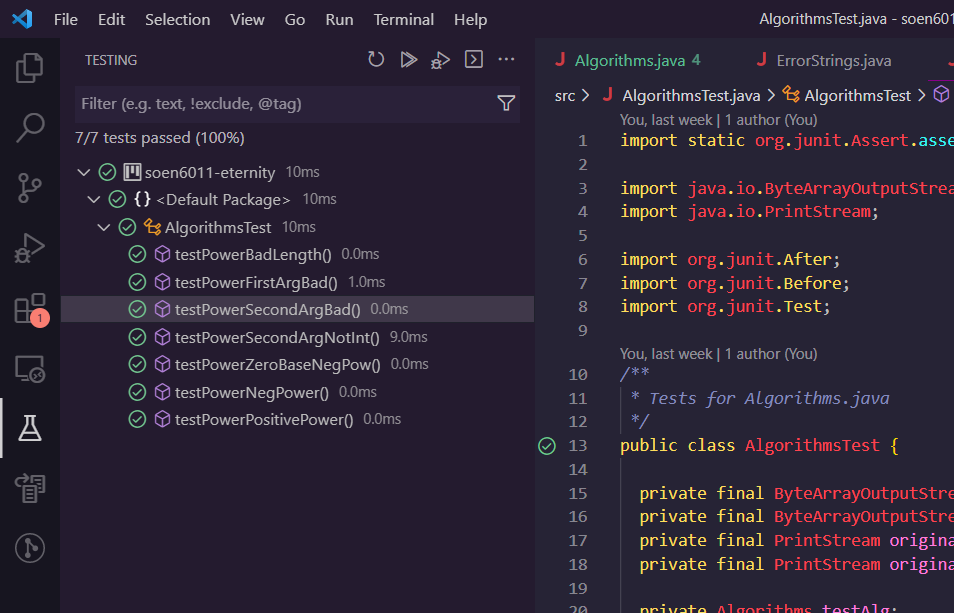
\includegraphics[width=\linewidth]{passed_test_cases.PNG}
            \caption{Execution of test cases on vs code.}
            \label{fig:passed_test_cases}
        \end{figure}
        
    All the tests are available in \href{https://github.com/akhil-sharma/soen6011-eternity/blob/main/src/AlgorithmsTest.java}{this} file on github.
    
    \appendix
        \chapter{Proof of compilation}
            \begin{figure}[htbp]
                \centering
                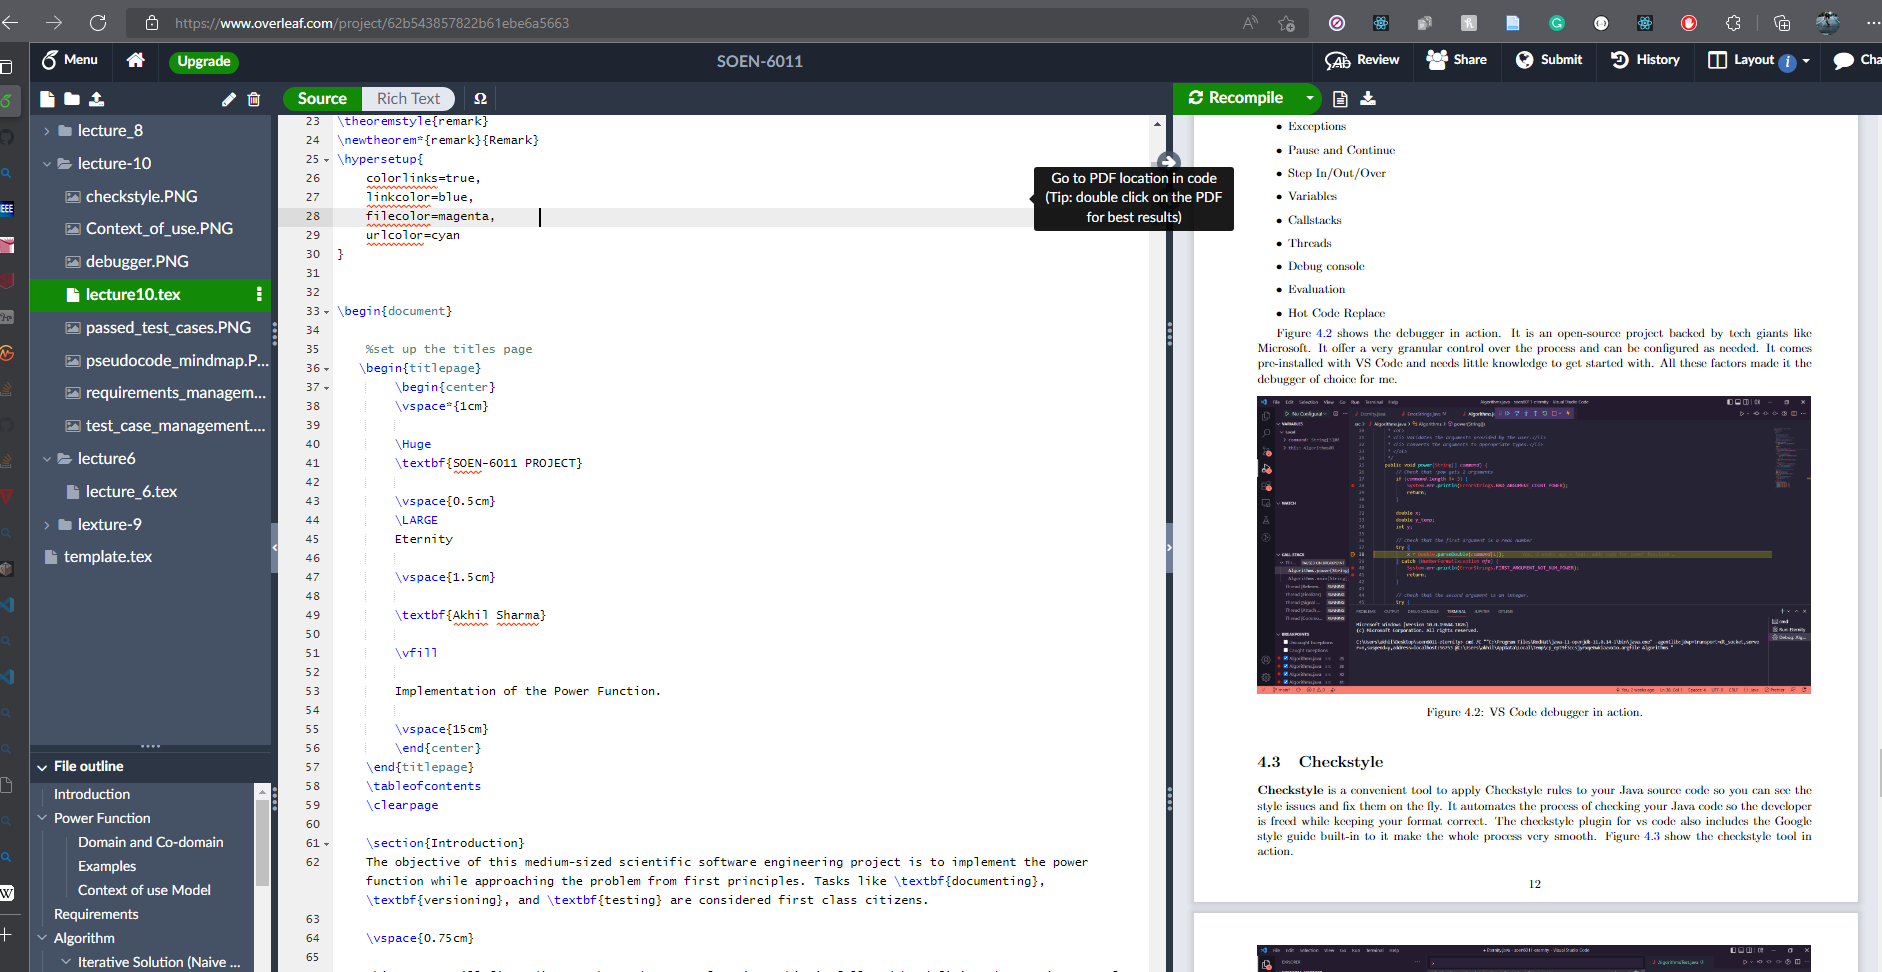
\includegraphics[width=\linewidth]{proof_of_compilation_online.PNG}
                \caption{Proof of compilation online at overleaf.com}
                \label{fig:proof_of_compilation_online}
            \end{figure}
            
            \begin{figure}[htbp]
                \centering
                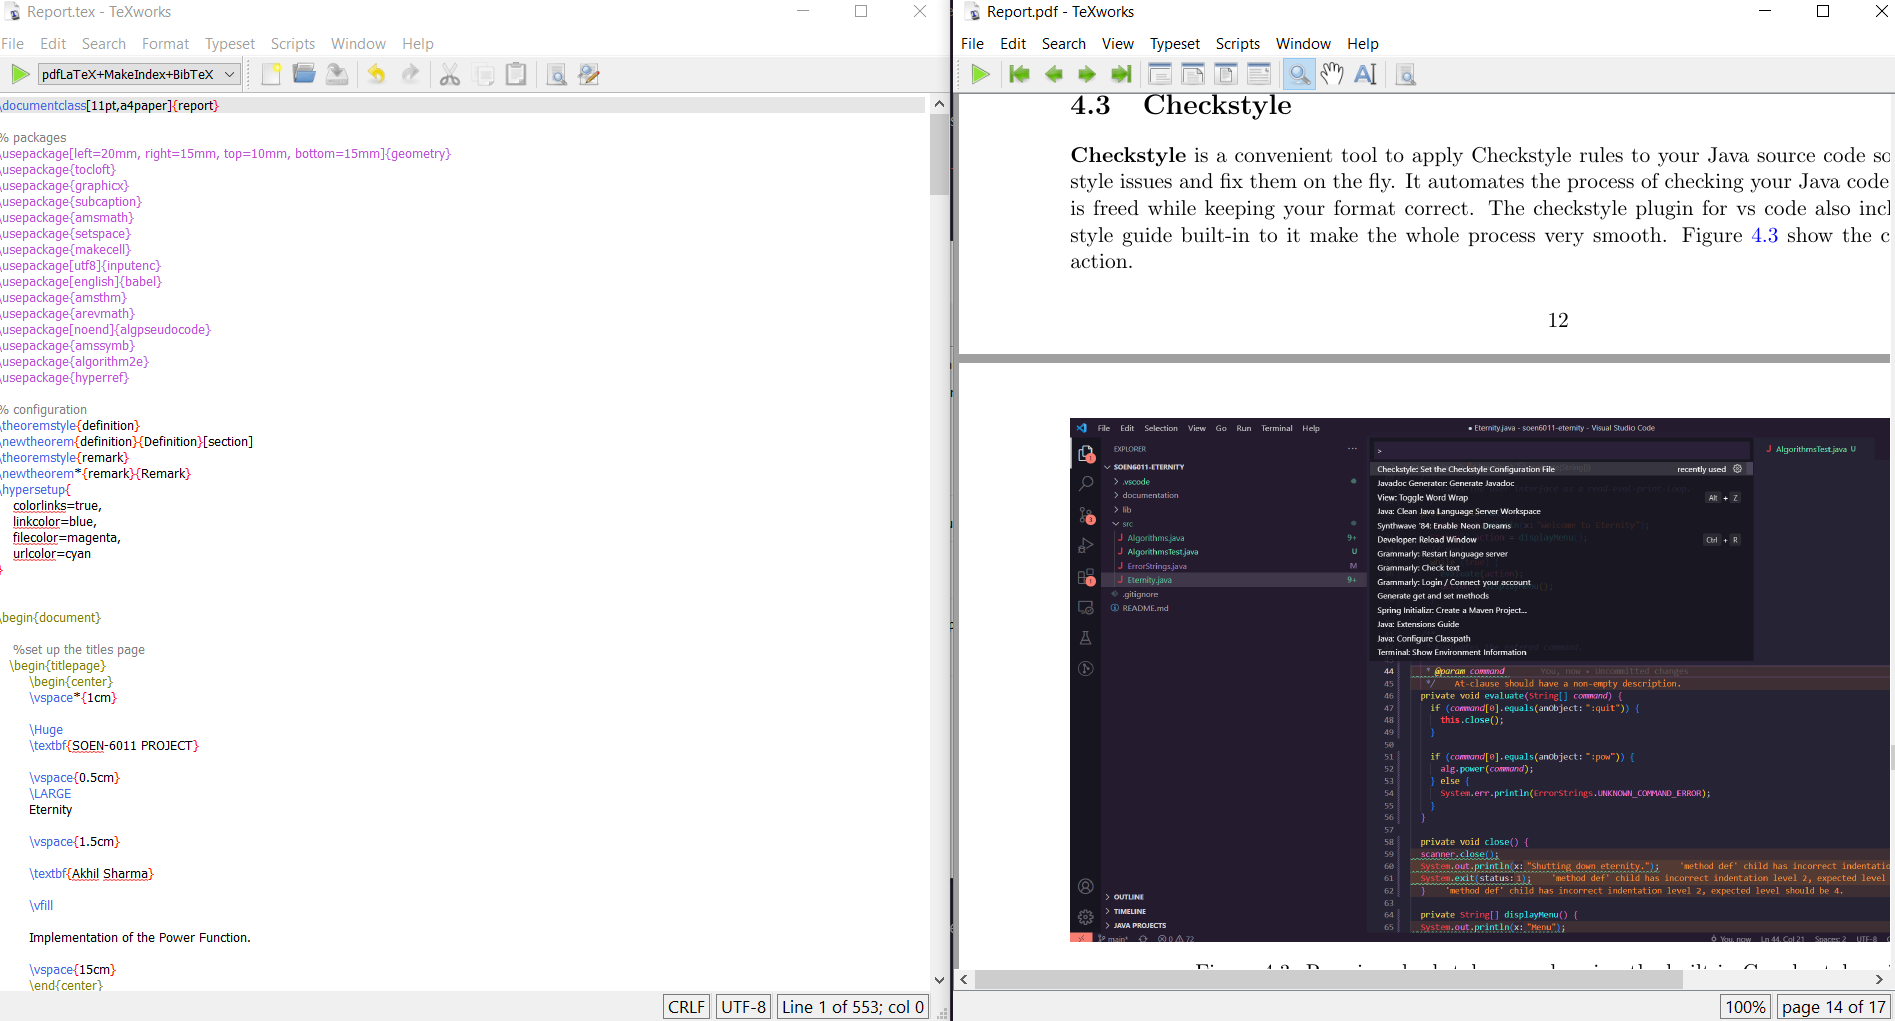
\includegraphics[width=\linewidth]{proof_of_compilation_offline.PNG}
                \caption{Proof of compilation offline on MikTex for windows.}
                \label{fig:proof_of_compilation_offline}
            \end{figure}
    
    \begin{thebibliography}{}
       \bibitem{algorithms}
       The Algebra Help e-book
       \url{https://mathonweb.com/help_ebook/html/functions_5.htm#power}
        
        \bibitem{context diagrams}
        What is a Context Diagram – Explain with Examples
        \url{https://www.edrawmax.com/context-diagram/}
        
    
    \end{thebibliography}
    
\end{document}